
%% bare_conf_compsoc.tex
%% V1.4b
%% 2015/08/26
%% by Michael Shell
%% See:
%% http://www.michaelshell.org/
%% for current contact information.
%%
%% This is a skeleton file demonstrating the use of IEEEtran.cls
%% (requires IEEEtran.cls version 1.8b or later) with an IEEE Computer
%% Society conference paper.
%%
%% Support sites:
%% http://www.michaelshell.org/tex/ieeetran/
%% http://www.ctan.org/pkg/ieeetran
%% and
%% http://www.ieee.org/

%%*************************************************************************
%% Legal Notice:
%% This code is offered as-is without any warranty either expressed or
%% implied; without even the implied warranty of MERCHANTABILITY or
%% FITNESS FOR A PARTICULAR PURPOSE! 
%% User assumes all risk.
%% In no event shall the IEEE or any contributor to this code be liable for
%% any damages or losses, including, but not limited to, incidental,
%% consequential, or any other damages, resulting from the use or misuse
%% of any information contained here.
%%
%% All comments are the opinions of their respective authors and are not
%% necessarily endorsed by the IEEE.
%%
%% This work is distributed under the LaTeX Project Public License (LPPL)
%% ( http://www.latex-project.org/ ) version 1.3, and may be freely used,
%% distributed and modified. A copy of the LPPL, version 1.3, is included
%% in the base LaTeX documentation of all distributions of LaTeX released
%% 2003/12/01 or later.
%% Retain all contribution notices and credits.
%% ** Modified files should be clearly indicated as such, including  **
%% ** renaming them and changing author support contact information. **
%%*************************************************************************


% *** Authors should verify (and, if needed, correct) their LaTeX system  ***
% *** with the testflow diagnostic prior to trusting their LaTeX platform ***
% *** with production work. The IEEE's font choices and paper sizes can   ***
% *** trigger bugs that do not appear when using other class files.       ***                          ***
% The testflow support page is at:
% http://www.michaelshell.org/tex/testflow/



\documentclass[conference,compsoc]{IEEEtran}
% Some/most Computer Society conferences require the compsoc mode option,
% but others may want the standard conference format.
%
% If IEEEtran.cls has not been installed into the LaTeX system files,
% manually specify the path to it like:
% \documentclass[conference,compsoc]{../sty/IEEEtran}





% Some very useful LaTeX packages include:
% (uncomment the ones you want to load)


% *** MISC UTILITY PACKAGES ***
%
%\usepackage{ifpdf}
% Heiko Oberdiek's ifpdf.sty is very useful if you need conditional
% compilation based on whether the output is pdf or dvi.
% usage:
% \ifpdf
%   % pdf code
% \else
%   % dvi code
% \fi
% The latest version of ifpdf.sty can be obtained from:
% http://www.ctan.org/pkg/ifpdf
% Also, note that IEEEtran.cls V1.7 and later provides a builtin
% \ifCLASSINFOpdf conditional that works the same way.
% When switching from latex to pdflatex and vice-versa, the compiler may
% have to be run twice to clear warning/error messages.






% *** CITATION PACKAGES ***
%
\ifCLASSOPTIONcompsoc
  % IEEE Computer Society needs nocompress option
  % requires cite.sty v4.0 or later (November 2003)
  \usepackage[nocompress]{cite}
\else
  % normal IEEE
  \usepackage{cite}
\fi
% cite.sty was written by Donald Arseneau
% V1.6 and later of IEEEtran pre-defines the format of the cite.sty package
% \cite{} output to follow that of the IEEE. Loading the cite package will
% result in citation numbers being automatically sorted and properly
% "compressed/ranged". e.g., [1], [9], [2], [7], [5], [6] without using
% cite.sty will become [1], [2], [5]--[7], [9] using cite.sty. cite.sty's
% \cite will automatically add leading space, if needed. Use cite.sty's
% noadjust option (cite.sty V3.8 and later) if you want to turn this off
% such as if a citation ever needs to be enclosed in parenthesis.
% cite.sty is already installed on most LaTeX systems. Be sure and use
% version 5.0 (2009-03-20) and later if using hyperref.sty.
% The latest version can be obtained at:
% http://www.ctan.org/pkg/cite
% The documentation is contained in the cite.sty file itself.
%
% Note that some packages require special options to format as the Computer
% Society requires. In particular, Computer Society  papers do not use
% compressed citation ranges as is done in typical IEEE papers
% (e.g., [1]-[4]). Instead, they list every citation separately in order
% (e.g., [1], [2], [3], [4]). To get the latter we need to load the cite
% package with the nocompress option which is supported by cite.sty v4.0
% and later.





% *** GRAPHICS RELATED PACKAGES ***
%
\ifCLASSINFOpdf
  % \usepackage[pdftex]{graphicx}
  % declare the path(s) where your graphic files are
  % \graphicspath{{../pdf/}{../jpeg/}}
  % and their extensions so you won't have to specify these with
  % every instance of \includegraphics
  % \DeclareGraphicsExtensions{.pdf,.jpeg,.png}
\else
  % or other class option (dvipsone, dvipdf, if not using dvips). graphicx
  % will default to the driver specified in the system graphics.cfg if no
  % driver is specified.
  % \usepackage[dvips]{graphicx}
  % declare the path(s) where your graphic files are
  % \graphicspath{{../eps/}}
  % and their extensions so you won't have to specify these with
  % every instance of \includegraphics
  % \DeclareGraphicsExtensions{.eps}
\fi
% graphicx was written by David Carlisle and Sebastian Rahtz. It is
% required if you want graphics, photos, etc. graphicx.sty is already
% installed on most LaTeX systems. The latest version and documentation
% can be obtained at: 
% http://www.ctan.org/pkg/graphicx
% Another good source of documentation is "Using Imported Graphics in
% LaTeX2e" by Keith Reckdahl which can be found at:
% http://www.ctan.org/pkg/epslatex
%
% latex, and pdflatex in dvi mode, support graphics in encapsulated
% postscript (.eps) format. pdflatex in pdf mode supports graphics
% in .pdf, .jpeg, .png and .mps (metapost) formats. Users should ensure
% that all non-photo figures use a vector format (.eps, .pdf, .mps) and
% not a bitmapped formats (.jpeg, .png). The IEEE frowns on bitmapped formats
% which can result in "jaggedy"/blurry rendering of lines and letters as
% well as large increases in file sizes.
%
% You can find documentation about the pdfTeX application at:
% http://www.tug.org/applications/pdftex





% *** MATH PACKAGES ***
%
\usepackage{amsmath}
% A popular package from the American Mathematical Society that provides
% many useful and powerful commands for dealing with mathematics.
%
% Note that the amsmath package sets \interdisplaylinepenalty to 10000
% thus preventing page breaks from occurring within multiline equations. Use:
%\interdisplaylinepenalty=2500
% after loading amsmath to restore such page breaks as IEEEtran.cls normally
% does. amsmath.sty is already installed on most LaTeX systems. The latest
% version and documentation can be obtained at:
% http://www.ctan.org/pkg/amsmath





% *** SPECIALIZED LIST PACKAGES ***
%
\usepackage{algorithmic}
% algorithmic.sty was written by Peter Williams and Rogerio Brito.
% This package provides an algorithmic environment fo describing algorithms.
% You can use the algorithmic environment in-text or within a figure
% environment to provide for a floating algorithm. Do NOT use the algorithm
% floating environment provided by algorithm.sty (by the same authors) or
% algorithm2e.sty (by Christophe Fiorio) as the IEEE does not use dedicated
% algorithm float types and packages that provide these will not provide
% correct IEEE style captions. The latest version and documentation of
% algorithmic.sty can be obtained at:
% http://www.ctan.org/pkg/algorithms
% Also of interest may be the (relatively newer and more customizable)
% algorithmicx.sty package by Szasz Janos:
% http://www.ctan.org/pkg/algorithmicx




% *** ALIGNMENT PACKAGES ***
%
\usepackage{array}
% Frank Mittelbach's and David Carlisle's array.sty patches and improves
% the standard LaTeX2e array and tabular environments to provide better
% appearance and additional user controls. As the default LaTeX2e table
% generation code is lacking to the point of almost being broken with
% respect to the quality of the end results, all users are strongly
% advised to use an enhanced (at the very least that provided by array.sty)
% set of table tools. array.sty is already installed on most systems. The
% latest version and documentation can be obtained at:
% http://www.ctan.org/pkg/array


% IEEEtran contains the IEEEeqnarray family of commands that can be used to
% generate multiline equations as well as matrices, tables, etc., of high
% quality.




% *** SUBFIGURE PACKAGES ***
%\ifCLASSOPTIONcompsoc
%  \usepackage[caption=false,font=footnotesize,labelfont=sf,textfont=sf]{subfig}
%\else
%  \usepackage[caption=false,font=footnotesize]{subfig}
%\fi
% subfig.sty, written by Steven Douglas Cochran, is the modern replacement
% for subfigure.sty, the latter of which is no longer maintained and is
% incompatible with some LaTeX packages including fixltx2e. However,
% subfig.sty requires and automatically loads Axel Sommerfeldt's caption.sty
% which will override IEEEtran.cls' handling of captions and this will result
% in non-IEEE style figure/table captions. To prevent this problem, be sure
% and invoke subfig.sty's "caption=false" package option (available since
% subfig.sty version 1.3, 2005/06/28) as this is will preserve IEEEtran.cls
% handling of captions.
% Note that the Computer Society format requires a sans serif font rather
% than the serif font used in traditional IEEE formatting and thus the need
% to invoke different subfig.sty package options depending on whether
% compsoc mode has been enabled.
%
% The latest version and documentation of subfig.sty can be obtained at:
% http://www.ctan.org/pkg/subfig




% *** FLOAT PACKAGES ***
%
%\usepackage{fixltx2e}
% fixltx2e, the successor to the earlier fix2col.sty, was written by
% Frank Mittelbach and David Carlisle. This package corrects a few problems
% in the LaTeX2e kernel, the most notable of which is that in current
% LaTeX2e releases, the ordering of single and double column floats is not
% guaranteed to be preserved. Thus, an unpatched LaTeX2e can allow a
% single column figure to be placed prior to an earlier double column
% figure.
% Be aware that LaTeX2e kernels dated 2015 and later have fixltx2e.sty's
% corrections already built into the system in which case a warning will
% be issued if an attempt is made to load fixltx2e.sty as it is no longer
% needed.
% The latest version and documentation can be found at:
% http://www.ctan.org/pkg/fixltx2e


%\usepackage{stfloats}
% stfloats.sty was written by Sigitas Tolusis. This package gives LaTeX2e
% the ability to do double column floats at the bottom of the page as well
% as the top. (e.g., "\begin{figure*}[!b]" is not normally possible in
% LaTeX2e). It also provides a command:
%\fnbelowfloat
% to enable the placement of footnotes below bottom floats (the standard
% LaTeX2e kernel puts them above bottom floats). This is an invasive package
% which rewrites many portions of the LaTeX2e float routines. It may not work
% with other packages that modify the LaTeX2e float routines. The latest
% version and documentation can be obtained at:
% http://www.ctan.org/pkg/stfloats
% Do not use the stfloats baselinefloat ability as the IEEE does not allow
% \baselineskip to stretch. Authors submitting work to the IEEE should note
% that the IEEE rarely uses double column equations and that authors should try
% to avoid such use. Do not be tempted to use the cuted.sty or midfloat.sty
% packages (also by Sigitas Tolusis) as the IEEE does not format its papers in
% such ways.
% Do not attempt to use stfloats with fixltx2e as they are incompatible.
% Instead, use Morten Hogholm'a dblfloatfix which combines the features
% of both fixltx2e and stfloats:
%
% \usepackage{dblfloatfix}
% The latest version can be found at:
% http://www.ctan.org/pkg/dblfloatfix




% *** PDF, URL AND HYPERLINK PACKAGES ***
%
\usepackage{url}
% url.sty was written by Donald Arseneau. It provides better support for
% handling and breaking URLs. url.sty is already installed on most LaTeX
% systems. The latest version and documentation can be obtained at:
% http://www.ctan.org/pkg/url
% Basically, \url{my_url_here}.

\usepackage{svg}
\usepackage{amsfonts}
\usepackage{bm}
\usepackage{hyperref}
\usepackage{epigraph}
\usepackage{booktabs}
\usepackage{enumitem}
\usepackage{float}
%\usepackage[keeplastbox]{flushend}
\usepackage{multirow}
\usepackage{tikz}


% *** Do not adjust lengths that control margins, column widths, etc. ***
% *** Do not use packages that alter fonts (such as pslatex).         ***
% There should be no need to do such things with IEEEtran.cls V1.6 and later.
% (Unless specifically asked to do so by the journal or conference you plan
% to submit to, of course. )


% correct bad hyphenation here
\hyphenation{op-tical net-works semi-conduc-tor}


\begin{document}
%
% paper title
% Titles are generally capitalized except for words such as a, an, and, as,
% at, but, by, for, in, nor, of, on, or, the, to and up, which are usually
% not capitalized unless they are the first or last word of the title.
% Linebreaks \\ can be used within to get better formatting as desired.
% Do not put math or special symbols in the title.
\title{A Comparative Study of Deep Learning Approaches in Off-Line Network Intrusion Detection
\footnote{The codebase for our project is available on https://github.com/littlepretty/NetLearner}}


% author names and affiliations
% use a multiple column layout for up to three different
% affiliations
\author{
\IEEEauthorblockN{Jiaqi Yan}
\IEEEauthorblockA{Department of Computer Science\\
Illinois Institute of Technology\\
Chicago, Illinois 60616\\
Email: jyan31@hawk.iit.edu}
\and
\IEEEauthorblockN{Jin Dong}
\IEEEauthorblockA{Department of Computer Science\\
Illinois Institute of Technology\\
Chicago, Illinois 60616\\
Email: dong.jin@iit.edu}
}

% conference papers do not typically use \thanks and this command
% is locked out in conference mode. If really needed, such as for
% the acknowledgment of grants, issue a \IEEEoverridecommandlockouts
% after \documentclass

% for over three affiliations, or if they all won't fit within the width
% of the page (and note that there is less available width in this regard for
% compsoc conferences compared to traditional conferences), use this
% alternative format:
% 
%\author{\IEEEauthorblockN{Michael Shell\IEEEauthorrefmark{1},
%Homer Simpson\IEEEauthorrefmark{2},
%James Kirk\IEEEauthorrefmark{3}, 
%Montgomery Scott\IEEEauthorrefmark{3} and
%Eldon Tyrell\IEEEauthorrefmark{4}}
%\IEEEauthorblockA{\IEEEauthorrefmark{1}School of Electrical and Computer Engineering\\
%Georgia Institute of Technology,
%Atlanta, Georgia 30332--0250\\ Email: see http://www.michaelshell.org/contact.html}
%\IEEEauthorblockA{\IEEEauthorrefmark{2}Twentieth Century Fox, Springfield, USA\\
%Email: homer@thesimpsons.com}
%\IEEEauthorblockA{\IEEEauthorrefmark{3}Starfleet Academy, San Francisco, California 96678-2391\\
%Telephone: (800) 555--1212, Fax: (888) 555--1212}
%\IEEEauthorblockA{\IEEEauthorrefmark{4}Tyrell Inc., 123 Replicant Street, Los Angeles, California 90210--4321}}


% use for special paper notices
%\IEEEspecialpapernotice{(Invited Paper)}


% make the title area
\maketitle

% As a general rule, do not put math, special symbols or citations
% in the abstract
\begin{abstract}
[Network intrusion detection is complex and needs to be A.I.]
Recently a handful of novel deep neural networks bundled with more advanced and smarter
training algorithms have achieved unprecedentedly good performance on image classification,
natural language processing, speech recognition and many other research branches.
Motivated by these impressive improvements in the field of artificial intelligence,
this paper tries to answer the following questions:
Can we transfer hall-of-fame deep learning approaches to network intrusion detection task?
If yes, how much improvement can be expected?
If no, what are the reasons?
We answer these questions in three steps.
Firstly, we introduce deep learning models and techniques and why they may better solve the
network intrusion detection problem from a high-level point of view.
Besides, we also survey and discuss the status quo of available network intrusion detection datasets
and its implication on applying deep learning models to network intrusion detection.
Then we briefly review the existing traditional machine learning approaches, some of which do but
some of which don't fit into the category of deep learning.
Nevertheless, these existing works provide the state-of-the-art detection performance.
In contrast to these approaches, we describe several groups of the cutting-edge deep learning models
in concisely mathematical languages.
We conduct a quantitatively comparative study of them with the off-line network intrusion detection datasets,
on the basis of our own TensorFlow-based deep learning library, NetLearner, that contains
multi-layer perceptrons, restricted Boltzmann machine, autoencoders and generative adversarial nets.
Apart from making NetLearner publicly available, we also share the hacks and tricks
used during the training phase so that future researchers can easily reproduce and extend our work.
[To the best of our knowledge, our feed-forward neural network achieves the best 5-classification
    result, with accuracy of 81.42\% and F1-Score of 80.44\%.]
\end{abstract}

% no keywords




% For peer review papers, you can put extra information on the cover
% page as needed:
% \ifCLASSOPTIONpeerreview
% \begin{center} \bfseries EDICS Category: 3-BBND \end{center}
% \fi
%
% For peerreview papers, this IEEEtran command inserts a page break and
% creates the second title. It will be ignored for other modes.
\IEEEpeerreviewmaketitle

\section{Introduction}

Network intrusion detection system (NIDS) is the essential security technology that
aims to protect a computer network intelligently and automatically.
As either a hardware device or software application,
it monitors a network for malicious activities or policy violations.
By intercepting and analyzing the bi-direction traffics through the network,
it raises alarm if intrusion, attack or violation are observed.
There are two general approaches to detect intrusions.
In signature based intrusion detection, e.g. SNORT~\cite{Snort},
rules for specific attacks are pre-installed in the system.
It report suspicious traffic when the traffic matches any signature of known attacks.
The major drawback of signature matching approach is that
it is only effective for previously detected attacks that have an identifiable signature.
As a result, signature database needs to be manually updated whenever a new type of attack
is discovered, with significant effort, by the network administrator.
Anomaly detection based approach overcomes these limitations by adopting a certain
type of machine learning technique to model the trustworthy network activities.
Traffics that significantly deviates from the built model are treated as malicious.
This idea have been shown to be able to detect unknown or novel attacks~\cite{NSL-KDD, STL-NIDS}.
However, if the built model for normal traffics are not generalized enough,
anomaly based approach will treat unforeseen normal traffic as malicious,
suffering from high false positive.

In this project, we follow the anomaly detection based idea, and tries to enhance it with the
state-of-art machine learning technology, e.g. various deep learning architectures.
Specifically, we have made the following contributions:
\begin{itemize}
    \item Firstly, we introduce the background of deep learning models and techniques,
        and discuss why they may better solve the network intrusion detection problem.
    %Besides, we also survey and discuss the status quo of available network intrusion detection datasets
    %and its implication on applying deep learning models to network intrusion detection.
    \item Then we briefly review the existing state-of-the-art machine learning solutions to network intrusion detection.
        After that, we describe several groups of the cutting-edge deep learning models
        in concisely mathematical languages.
    \item We conduct a quantitatively comparative study of each of them with
        two off-line network intrusion detection datasets~\cite{NSL-KDD, UNSW},
        with the help of our own TensorFlow-based deep learning library, NetLeaner.
        The detection performance is measured in accuracy, precision, recall and F-Score,
        with detailed confusion matrix.
\end{itemize}

We not only make the codebase of NetLearner publicly available to research community,
but also share the deep learning related hacks and tricks used during the training phase,
so that future researches can easily reproduce and extend our work.

\section{Deep Learning Background}
We identify three main reasons why deep learning succeed in many areas that related
to artificial intelligence, as well as their implications on network intrusion detection problem.

\subsection{Learning/Training Techniques}
Given the feature representations and machine learning or neural network model,
learning is in essential an optimization problem which minimizes a predefined loss function over given training examples.
The most commonly used optimization algorithm is back-propagation(BP)~\cite{Backpropagation} with gradient descent,
because the computing gradient is Hessian-free and memoization saves a great amount of computation when
back propagating level by level.
However, it is impossible to train deep neural networks and achieve optimal parameters only with BP.
The first problem is that usually the cost function is non-convex with a lot of local minima and
first-order gradient is very easy to stuck at a poor local minimum.
Secondly, exploding and vanishing gradient will make back-propagation difficult to train models with many layers stacked together, such as recurrent neural networks and stacked Restricted Boltzmann Machines.
Even if we can tolerate the long training time and carefully deal with gradient exploding and vanishing,
the trained model is usually overfitted to the training dataset, and not able to generalize well to the testing or future dataset.

The emergence of many novel learning algorithms and training techniques makes training large and deep
neural network and achieving good suboptimal minimum possible.
For example, stochastic gradient descent (SGD) with mini-batches can greatly increase the training speed comparing
to normal gradient descent the entire dataset.
In each step of gradient descent, researchers have shown that momentum~\cite{Momentum} can
prevent SGD from oscillating across but pushing along the shallow ravine.
Along with decaying learning rate, momentum-based optimization algorithms, for example Adam~\cite{Adam},
usually help us find better local minimum.
To prevent overfitting, researchers have proposed dropout~\cite{Dropout} to average over
exponential number of neural network models.
These learning algorithms and training techniques will directly help neural networks achieve
better performance for the network intrusion detection problem,
since they are general to any types of neural models.


\subsection{Unsupervised Generative Models}
Another breakthrough in the deep learning area is that researchers have successfully trained
a number of novel unsupervised generative models that attracted much attentions.
Different from supervised models (or discriminative models) that tries to discover the relationship between input variables and target label (or the conditional probability distribution of the targets given the input),
these models aims to learn the joint probability distribution, or joint conditional distribution,
of \textbf{all} variables for a phenomenon from the given dataset.
The resulting generative model is powerful in many ways.
First, given the well trained probability distribution, the model can synthesize meaningful data
comparable to real examples in training set.
For example, Auxiliary-Classifier Generative Adversarial Nets (AC-GAN)~\cite{AC-GAN} can generate very high quality
images after training on ImageNet dataset~\cite{ImageNet};
both stacked denoising autoencoder~\cite{DenoiseAE} and deep brief nets~\cite{DeepBeliefNets} can synthesize
handwritten digits after learning from the MNIST dataset.
Besides, the ability to generate meaningful and high quality faked data actually means that
the model have learned better feature representations from the unlabeled data itself.
As an example, it is shown that the features extracted from the hidden units of sparse autoencoder
can significantly improve the performance of support vector classifier~\cite{SparseAE}.
At last, researchers have shown that it is usually a good strategy to initialize deep neural networks
with the weights from a successfully trained generative model~\cite{DeepBeliefNets, Momentum}.

In the area of network security, the amount of network traffic data is enormously large,
usually in the order of terabytes per day in a large monitored network.
In practice, the amount of data is impossible for a human security analyst or
a group of them to review, e.g., to find patterns and label anomalies.
This situation makes an unsupervised generative model a promisingly good solution
to traffic classification since it can be trained unsupervised:
\begin{itemize}
    \item It utilizes the large amount of unlabeled data to learning useful and hierarchical features
        from the data itself;
    \item It is equivalently a way to initialize the weights of the hidden layers
        in a deep neural network, which can be further fine-tuned to be a high performance classifier.
\end{itemize}
In this project we propose to try three types of generative models:
restricted Boltzmann machine, autoencoders and generative adversarial nets.

\subsection{Datasets}

\begin{table*}[]
\centering
\caption{Popular Datasets used in Deep Learning v.s. Available Network Traffic Datasets}
\label{Tab:Datasets}
\begin{tabular}{c|c|c|c|c}
\multicolumn{1}{c|}{Domain}                          & Dataset Name  & \#Examples in Training Set & Feature Dimension                         & Dataset Size \\
\hline
\hline
\multirow{6}{*}{Image}                               & MNIST         & 60,000        & 784 (28$\times$28 gray images)            & 47.04 million \\
                                                     & SVHN          & 600,000       & 3072 (32$\times$32 color images)          & 1843.2 million \\
                                                     & CIFAR-10      & 60,000        & 3072 (32$\times$32 color images)          & 184.32 million \\
                                                     & Flickr Photo  & 100 million   & $\geq$16,000 RGB pixels per image          & $\geq$48 trillion \\
                                                     & Tiny          & 80 million    & $\geq$256 RGB pixels per image             & $\geq$20.48 billion \\
                                                     & ImageNet      & 100 million   & $\geq$49,152 (128$\times$128 color images) & $\geq$4.91 trillion \\
\hline
\multicolumn{1}{l|}{\multirow{2}{*}{Network Traffic}} & UNSW-NB15    & 175,341       & 42                                        & 7.36 million \\
\multicolumn{1}{l|}{}                                 & NSL-KDD      & 125,973       & 41                                        & 5.16 million
\end{tabular}
\end{table*}

\section{Existing Works}
Due to the large number of network intrusion detection systems that adopt machine learning or data mining approaches
we only review a few of them that achieve state-of-the-art detection performance.
There are very limited number of existing network intrusion detection systems that adopt
deep learning approaches.
Their details can be found in section~\ref{Sec:Architectures}.

\subsection{State-of-Art Machine Learning Approaches}
Prior researchers modeled the intrusion detection task as an unsupervised
anomaly detection problem, and proposed a series of approaches.
Examples include Mahalanobis-distance based outliner detection~\cite{ComparativeAnomalyNIDS},
density-based outliner detection~\cite{LOF, ComparativeAnomalyNIDS},
evidence accumulation for ranking outliner~\cite{RankingOutliner}, etc.
One of the advantage of these unsupervised approaches is to tackle the problem of
the unavailability of labeled traffic data.

Alternatively, prior researchers made a lot of effort to obtain meaningful
attacking data and to convert them into labeled data~\cite{DARPA, KDDCup, NSL-KDD, UNSW, UNSW1}.
Such efforts make it possible to apply supervised machine learning algorithms to the
intrusion detection problem.
Successfully applied approaches include decision trees~\cite{DecisionTree},
linear and non-linear support vector machines~\cite{SVM}, NB-Tree~\cite{NB-Tree} and so on.
To the best of the authors' knowledge, there are two works that achieved the best prediction
accuracy on the two different datasets respectively.
For the UNSW-NB15 dataset, it is reported in~\cite{RampLossKSVCR} that extending K-support vector
classification-regression~\cite{KSVCR} with ramp loss, called Ramp-KSVCR approach, can achieve the state-of-the-art accuracy of 93.52\%.
The authors of Ramp-KSVCR also report that their approach can achieve 98.68\% accuracy on the NSL-KDD dataset.
On the other hand, the creators of UNSW-NB15 dataset~\cite{UNSW} proposed an approach called
Geometric Area Analysis techniques using trapezoidal area estimation (GAA-ADS for short)~\cite{GAA-ADS}.
It achieves the bese known accuracy on NSL-KDD dataset (99.7\%) and a slightly worse accuracy on
UNSW-NB15 dataset (92.8\%).


\subsection{Deep Learning Flavor Approaches}
There are some pioneer works that introduced deep learning approaches to intrusion detection.
For example, \cite{STL-NIDS} adopts sparse autoencoder and the self-taught learning
scheme~\cite{SparseAE} to handle the problem of limited amount of labeled data for training supervised model.
Similar semi-supervised approach have also been applied to
Discriminative restricted Boltzmann machine~\cite{AnomalyDetectionRBM}.

\section{Neural Networks}
In this section, we give a brief review of the deep learning architectures that we used
in the network intrusion detection problem.

\subsection{Multilayer Perceptron}
Multilayer perceptron (MLP) is a classic deep learning classifier with simple
design of the connectivity between neurons.
It is a fully connected feed-forward neural network, as shown in Figure~\ref{Fig:MLPArchitecture}.
By introducing non-linear neural units (perceptrons), it can distinguish data that are
not linearly separable.
However, the non-linearity also make it very hard to train a deep MLP of more than three layers,
even if people have proposed the efficient back-propagation learning algorithm~\cite{Backpropagation}.
Recently it revived due to the various new training techniques designed by deep learning community,
including Stochastic Gradient Descent (SGD),
batch normalization~\cite{BatchNorm} and Dropout~\cite{Dropout}.
Except for the number of neurons in each layer and number of layers,
MPL can also be tuned with different activation functions, or neural types.
The most popular two, which are used in this project, are logistic function
and rectifier linear unit.
Logistic function is written as
\begin{align}
    f(x) &= \frac{1}{1 + e^{-x}}
\end{align}
It has a very useful property when we applying back-propagation:
\begin{align}
    f'(x) &= f(x) (1-f(x))
\end{align}
Recently, most deep neural networks adopt rectifier neural unit and
achieved very good performance~\cite{DeepLearning}.
Rectifier linear unit is defined as
\begin{align}
    f(x) &= \max(0, x)
\end{align}
Let $\mathbf{a}^{(l)}$ be the activation of layer $l$,
$\mathbf{W}^{(l)}$ and $\mathbf{b}^{(l)}$ be layer $l$'s parameter.
With activation function defined, we have the following recursive formula that describes
the feed-forward step of the perceptron network.
\begin{align}
    \mathbf{z}^{(l+1)} &= \mathbf{W}^{(l)} \mathbf{a}^{(l)} + \mathbf{b}^{(l)} \label{Equ:MLPFeedForward1}\\
    \mathbf{a}^{(l+1)} &= f(\mathbf{z}^{(l+1)})
    \label{Equ:MLPFeedForward2}
\end{align}

\begin{figure}[h]
    \centering
    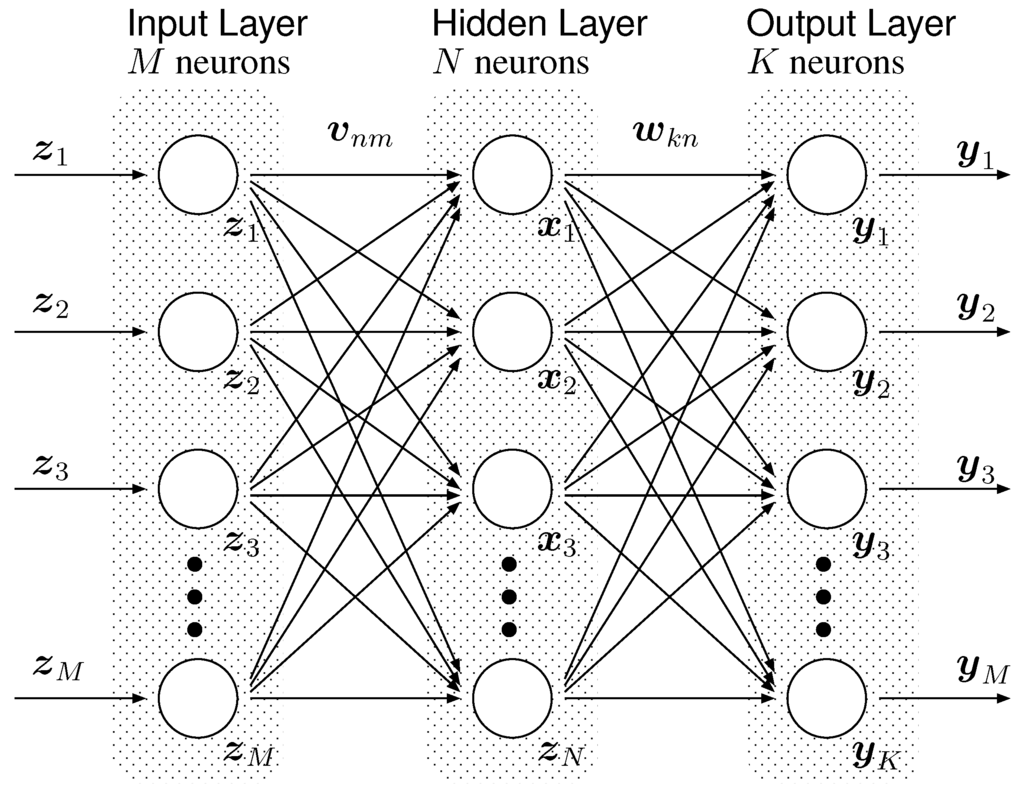
\includegraphics[width=0.45\textwidth]{figures/multilayer_perceptron.png}
    \caption{A multilayer perceptron neural network with 1 hidden layer.
        Figure courtesy of Teijiro Isokawa, Haruhiko Nishimura and Nobuyuki Matsui.}
    \label{Fig:MLPArchitecture}
\end{figure}

\subsection{Generative Models}
The amount of network traffic data is enormously large, usually in the order of terabytes
per day in a large monitored network.
Such available big data makes deep learning techniques a promisingly better solution
to traffic classification.
In practice, however, the amount of data is impossible for a human security analyst or
a group of them to review, e.g., to find patterns and label anomalies.
Generative model which can be trained unsupervised comes to rescue in that
\begin{itemize}
    \item It utilizes the large amount of unlabeled data to learning useful and hierarchical features
        from the data itself;
    \item It is equivalently a way to initialize the weights of the hidden layers
        in a deep neural network, which can be further fine-tuned to be a high performance classifier.
\end{itemize}
In this project we propose to try two generative models: restricted Boltzmann machine and autoencoders.

\subsubsection{Restricted Boltzmann Machine}
Restricted Boltzmann machine (RBM)~\cite{RBMTechReport} is a type of energy-based model,
which associate a scalar energy to each configuration vector of the variables in the network.
In energy-based model, learning is the process of configuring the network weights so that
the average energy over training data is minimized.
RBM consists of a layer of hidden units (H) and a layer of visible units (V).
Here ``restricted" means that connections are just between hidden and visible layer,
but not within hidden layers or visible layers.
This makes its training to be faster than Boltzmann machine and makes it feasible to
stack multiple separately trained RBM together to form deep architecture.
A joint configuration, $(\mathbf{v, h})$, of the visible and hidden units has the energy of
\begin{align}
    E(\mathbf{v, h}) &= -\sum_{i\in visible}a_i v_i - \sum_{j\in hidden}b_j h_j - \sum_{i, j}v_i h_j w_{ij}
\end{align}
where $a=\{a_i\}$ and $b=\{b_j\}$ are biases in visible and hidden layer respectively,
and $W=\{w_{ij}\}$ is the weights between them.
The network assigns a probability to every possible pair of $(\mathbf{v, h})$ via this energy
function
\begin{align}
    p(\mathbf{v, h}) &= \frac{1}{Z} e^{-E(\mathbf{v, h})} \\
    p(\mathbf{v}) &= \frac{1}{Z} \sum_{\mathbf{h}} e^{-E(\mathbf{v, h})}
\end{align}
where $Z$ is the partition function that equals to the summation over all possible hidden
and visible vector pairs
\begin{align}
    Z = \sum_{\mathbf{v,h}} e^{-E(\mathbf{v, h})}
\end{align}
Based on the ``maximizing log likelihood" idea,
we want to raise the probability of a training example and it can be done by
adjusting the weights biases to lower the energy of the considered example.
Meanwhile, we can let other examples make a big contribution to the partition function $Z$
by raising their energy.
Both insights can be translated to the following formula:
\begin{align}
    \frac{\partial \log p(v)}{\partial w_{ij}} = \langle v_i h_j \rangle_{data} - \langle v_i h_j \rangle_{model} 
\end{align}
This implies the following learning rule for performing stochastic gradient ascent on training
data
\begin{align}
    \Delta w_{ij} &= \varepsilon (\langle v_i h_j \rangle_{data} - \langle v_i h_j \rangle_{model})
\end{align}
The first term $\langle v_i h_j \rangle_{data}$ is the sampling from the data and it is easy to
compute since there is no directed connection between hidden units.
The sampling of $h_j$ is based on the probability
\begin{align}
    Prob(h_j = 1 | \mathbf{v}) &= sigmoid(b_j + \sum_i{v_i w_{ij}})
    \label{Equ:RBMSampleHidden}
\end{align}
Similarly, $v_i$ can be sampled with the following distribution
\begin{align}
    Prob(v_i = 1 | \mathbf{h}) &= sigmoid(a_j + \sum_j{h_i w_{ij}})
    \label{Equ:RBMSampleVisible}
\end{align}
The term $\langle v_i h_j \rangle_{model}$ can be obtained by performing alternative Gibbs
sampling for a long time.
The sampling starts from a random visible state.
Then we update the hidden units in parallel with Equation~\ref{Equ:RBMSampleHidden},
followed by updating the visible units in parallel with Equation~\ref{Equ:RBMSampleVisible}.
Instead of doing alternating Gibbs sampling for a large number of iterations,
\cite{TrainCD} proposed contrastive divergence (CD) as a faster learning procedure.
The training also start with a training vector to compute the states of the hidden units
using Equation~\ref{Equ:RBMSampleHidden}.
Then, with the chosen hidden states, we reconstruct the visible states by sampling each $v_i$
with probability given in Equation~\ref{Equ:RBMSampleVisible}.
The change of weight is then computed by
\begin{align}
    \Delta w_{ij} = \varepsilon (\langle v_i h_j \rangle_{data} -
    \langle v_i h_j \rangle_{reconstruct})
    \label{Equ:RBMCD1}
\end{align}
This is called contrastive divergence using one full step of alternating Gibbs sampling.
Contrastive divergence with $n$ rounds of alternating Gibbs sampling
is usually denoted as CD$n$.

The layer-by-layer training algorithm for stacking RBMs goes in a greedy fashion.
After learning the first layer RBM, the activity vector of the hidden units can be used
as ``data" for training the RBM in the second layer
and this process can be repeated to learn as many hidden layers as desired.
As data passing through the RBMs, we obtain the highest level features 
which are typically fed into a classifier.
The entire deep network (RBMs plus the classifier) can be fine-tuned to
improve the classification performance.


\begin{figure}[h]
    \centering
    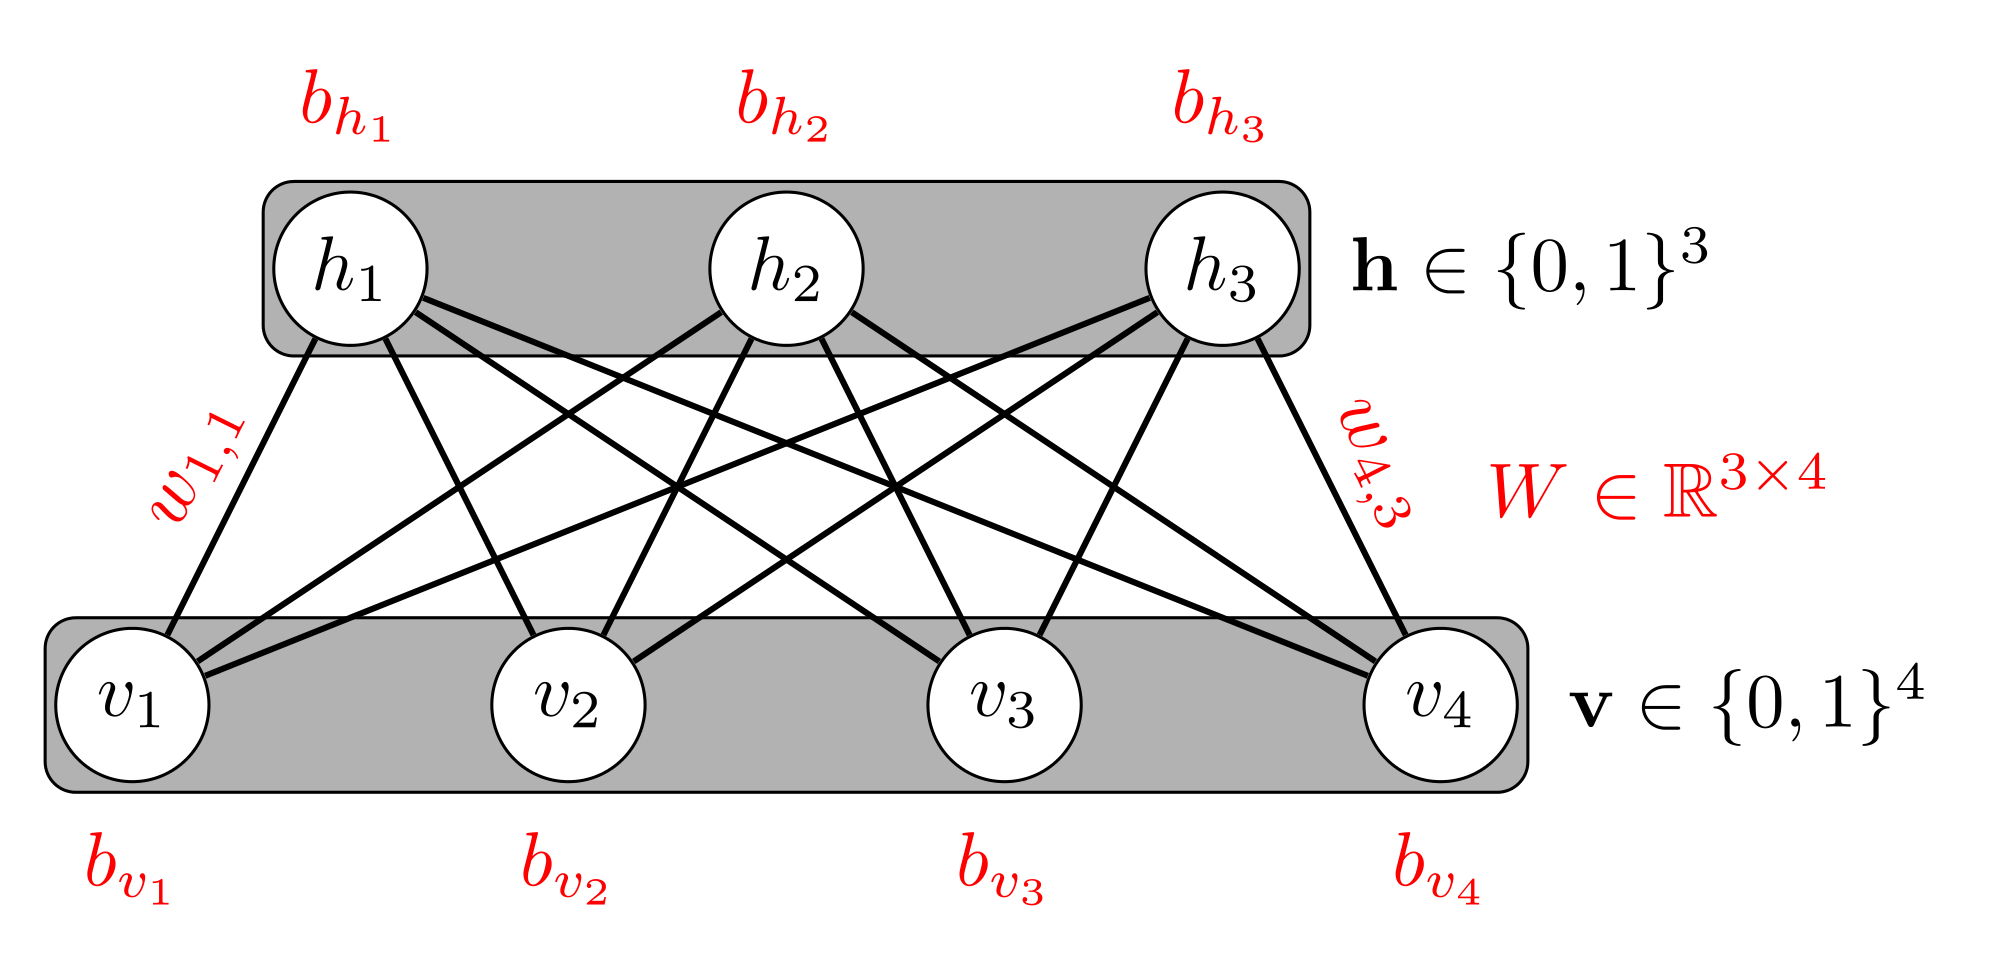
\includegraphics[width=0.45\textwidth]{figures/rbm.png}
    \caption{Restricted Boltzmann Machine.
        Figure courtesy of https://commons.wikimedia.org/wiki/File:Restricted-boltzmann-machine.svg}
    \label{Fig:RBMArchitecture}
\end{figure}



\subsubsection{Autoencoders}
An autoencoder neural network is an unsupervised model with typically one hidden layer that
tries to set the output layer to be equal to the input.
As shown in Figure~\ref{Fig:AEArchitecture}, we want the network to
learn a function $h_{W, b}(x) \approx x$.
However, to prevent the network from learning the meaningless identity function,
we need to place extra constraints on the network, giving birth to different
flavors of autoencoders.
In this project we consider two most popular types of autoencoder, sparse autoencoder and
denoising autoencoder.

The \textbf{denoising autoencoder} algorithm is proposed by~\cite{DenoiseAE} and illustrated in
Figure~\ref{Fig:dAEAlgorithm}.
To prevent learning identity function, an example $\mathbf{x}$ is first corrupted, either by
adding Gaussian noise or by random masking a fraction of items in $\mathbf{x}$ to zero.
The autoencoder then maps corrupted $\mathbf{\tilde{x}}$ to a hidden representation $\mathbf{y} = sigmoid(\mathbf{W}\tilde{\mathbf{x}} + \mathbf{b})$.
From $\mathbf{y}$ we reconstruct $\mathbf{z}=g_\theta'(\mathbf{y})$.
The training needs to learn the parameters $\theta$ and $\theta'$ so that
average reconstruction error is minimized over training set.
For binary input $\mathbf{x}$, usually cross entropy is adopted as $L_H(\mathbf{x}, \mathbf{z})$;
while mean squared error is used for real-valued $\mathbf{x}$.

\begin{figure}[h]
    \centering
    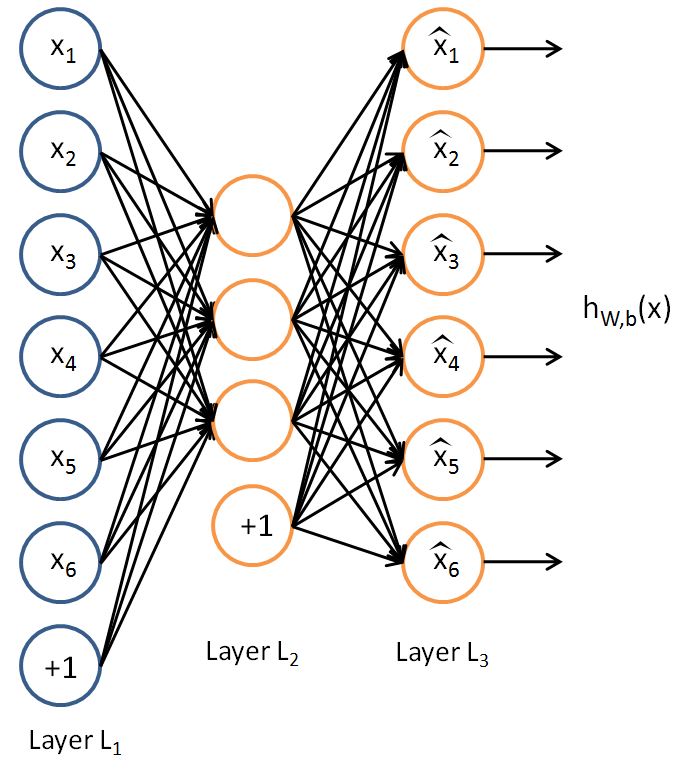
\includegraphics[width=0.45\textwidth]{figures/autoencoder.png}
    \caption{General Architecture of Autoencoders.
        Figure courtesy of~\cite{UFLDLAutoencoder}.}
    \label{Fig:AEArchitecture}
\end{figure}

\begin{figure}[h]
    \centering
    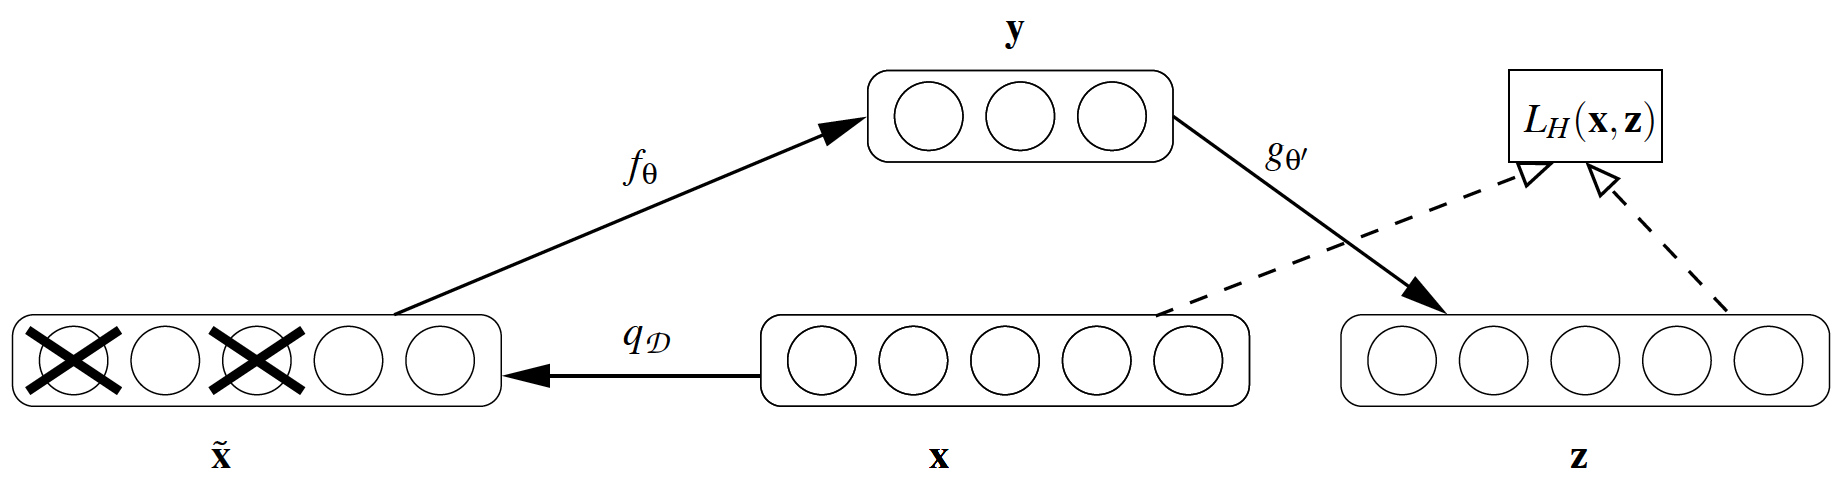
\includegraphics[width=0.45\textwidth]{figures/denoiseautoencoder.png}
        \caption{The denoising autoencoder algorithm.
        Input example $\mathbf{x}$ is randomly corrupted via $q_\mathcal{D}$ and then
        is mapped via encoder $f_\theta$ to $\mathbf{y}$.
        The decoder $g_\theta'$ attempts to reconstruct $\mathbf{x}$ and produces $\mathbf{z}$.
        Reconstruction error is measured by loss $L_H(\mathbf{x}, \mathbf{z})$, to be minimized
        during the training phase.
        Figure courtesy of~\cite{DenoiseAE}.}
    \label{Fig:dAEAlgorithm}
\end{figure}

The \textbf{sparse autoencoder} works by placing a sparsity constraint on the hidden units~\cite{SparseAE}.
First, we make the autoencoder's hidden layer size to be over-complete,
that is, of larger size comparing to the dimension of the input.
Let's denote the activation of hidden unit $j$ of layer 2 in Figure~\ref{Fig:AEArchitecture}
to be $a^2_j(\mathbf{x})$ given input example $\mathbf{x}$.
With that, we define the average activation of hidden unit $j$ over the $m$-size
training set
\begin{align}
    \hat{\rho}_j = \frac{1}{m} \sum_{i=1}^{m} a^2_j(\mathbf{x})
\end{align}
The sparsity constraint is enforcing, $\forall$ hidden unit $j$,
\begin{align}
    \hat{\rho}_j = \rho
\end{align}
where $\rho$ is a sparsity parameter that approximates zero (say 0.05).
This constraint can be vectorized over the hidden layer, say of size $n_2$,
with the KL divergence based penalty term
\begin{align}
    \sum_j^{n_2} KL(\rho || \hat{\rho}_j)
    = \sum_j^{n_2} [\rho \log \frac{\rho}{\hat{\rho}_j} + (1 - \rho) \log \frac{1-\rho}{1-\hat{\rho}_j} ]
\end{align}
The sparsity penalty term is integrated into the cost function by adding another hyper-parameter $\beta$
\begin{align}
    L(W, b) = \frac{1}{2}||h_{W,b}(\mathbf{x}) - \mathbf{x}||^2 +
    \beta \sum_j^{n_2} KL(\rho || \hat{\rho}_j)
\end{align}

Denoising autoencoder and sparse autoencoder, surprisingly, have different application domains.
Vincent et al.~\cite{DenoiseAE} have shown that stacked denoising autoencoder can be used to
initialize a deep neural network's weight parameter,
achieving similar and sometimes better performance than stacked RBM.
They also show that training stacked denoising autoencoder with MNIST dataset, it is able
to re-synthesize a variety of similarly good quality digits.
Raina et al.~\cite{SparseAE} have compared sparse encoding with principle component analysis
(PCA) and argue that transferring raw features with a well unsupervised trained
sparse autoencoder can be beneficial to supervised learning algorithms,
for example support vector machines (SVM).

\section{Implementation}

\subsection{TensorFlow 101}
TensorFlow~\cite{TensorFlow} is an open-source software library for machine learning
developed by the Google Brain Team.
The library models the computations in machine learning as data flow graphs.
Multidimensional data arrays are called tensors in TensorFlow.
Nodes in the graph represent mathematical operations between tensors,
such as add, multiply, softmax and dropout.
Graph edges represent the flow of tensors between nodes.
The computation graph based architecture allow researchers to run or train neural networks
on one or more CPUs or GPUs with unified API.

For general classification task, input $X$ and label $Y$ are defined as \textbf{placeholder}s
and feed into the computation graph at running time using a dictionary.
The graph of a typical deep learning model have three parts.
The \textbf{inference} graph should be built so that output predictions are returned as tensor.
For example, in the multilayer perceptron case, inference graph contains all iterative
computation~\ref{Equ:MLPFeedForward1}-\ref{Equ:MLPFeedForward2} in the feed-forwarding steps.
The \textbf{loss} graph should compute the loss function defined by specific models or algorithms.
Usually it is either cross-entropy or mean-squared error averaged across the batch data.
The loss graph will be optimized, usually minimized, by the \textbf{train} part.
This optimization can be conducted by various optimizing algorithms, such as gradient descent,
Momentum, RMSProp.
After sufficient steps of batch training, we evaluate the trained model with inference
graph and compare the predictions with the test dataset labels.
TensorFlow also provides various useful utilities for training models and running experiments.
Using a Saver, we are able to checkpoint the training process so as to restoring the model
for further training or evaluation.
Users create Summary nodes to log the snapshot of interest variables, which can be
automatically visualized by TensorBoard.

\subsection{NetLearner}
We provide a Python library NetLearner~\cite{NetLearner} that wraps up several deep learning models on the basis of TensorFlow.
NetLearner modularizes multilayer perceptron, restricted Boltzmann machine, sparse autoencoder
and masking-noise autoencoder, all of which are used to perform the 5-class classification
on the NSL-KDD dataset.

\subsection{Hacks and Tricks}
For the multiple layer perceptron, we tried a 4-hidden-layer network with
very wide size in each layer, several hundreds for each layer.
The accuracy on training set is very exiting, usually more than 96\%.
However, its performance on test dataset is not satisfactory.
Instead we found out that a single hidden layer with only sixteen neurons has good accuracy.
It is trained with stochastic gradient descent (SGD) for 20 epochs and batch size 100.
During the training, learning rate decays from 0.1 exponentially with the base of 0.32.
We did not include regularization in the model, but did apply dropout of keep probability 0.8.
We denote this approach as MLP and show its detailed results in the later section.

We build a RBM with 200-hidden units to perform unsupervised feature learning first on the dataset.
The learned features are then fed into a simple softmax regression classifier.
We trained the RBM using CD1 (contrastive divergence using one full step to get the negative data),
with batch size 10 for 40 epochs.
The learning rate is initialized at 0.01 and decay exponentially with the base of 0.64.
We denote this combination of RBM and softmax regression as RBM in the later section.

We also implemented the self-taught learning architecture proposed in~\cite{STL-NIDS, SparseAE},
adopting sparse autoencoder as the unsupervised feature learner.
The learned features will then be used for classification by a Softmax regression classifier.
We contact the author of~\cite{STL-NIDS} so that we can reproduce their implementation
with the same hyper-parameters.
For example, the hidden layer size of the sparse autoencoder is 64;
the sparsity value $\rho$ is 0.25.
Different from~\cite{STL-NIDS}, we found that using regularization in
neither autoencoder nor softmax regression is helpful.
So we didn't include regularization term in the both autoencoder and softmax cost function.
The autoencoder is trained with SGD for 1000 epochs and batch size 5000.
Different from MLP, we used Adam optimizer during the training.
The learning rate starts at 0.01 and decay exponentially with base of 0.6.
We denote this approach as SAE and report its performance in the later section.

As a variation to the sparse autoencoder based self-taught learning architecture,
we explore what will the performance be if we replace sparse autoencoder with denosing autoencoder.
We simply use dropout to emulate the masking noise and build masking noise autoencoder,
in which input is randomly masked out with keep probability of 0.4.
The size of the denoising autoencoder is 100.
The autoencoder is trained with SGD for 1000 epochs and batch size 5000.
We trained denoising autoencoder in the same way as we trained sparse autoencoder.
The result of this approach is labeled as DAE in the later section.

One thing to notice is that we use the same seed to randomly initialized the weights and biases
of the softmax regression classifier such that the learned features from RBM, sparse autoencoder and
denoising autoencoder are comparable.
For the same reason, all the softmax regression classifiers used by RBM, sparse autoencoder and
denoising autoencoder are trained with Adam optimizer of batch size 100 for 100 epochs,
with exponentially decay learning rate starting at 0.01,
with dropout technique of keep probability 0.8.


\section{Experiment Results}

\subsection{Dataset and Preprocessing}

Among alternative available datasets~\cite{KDDCup, DARPA, UNSW1},
we choose NSL-KDD dataset~\cite{NSL-KDD} and UNSW-NB15 dataset~\cite{UNSW}
to evaluate the performance of various proposed neural networks in the network intrusion detection.

\subsubsection{NSL-KDD Dataset}
The NSL-KDD dataset originates from the KDDCup 99 dataset~\cite{KDDCup},
which was used for the third International Knowledge Discovery and Data Mining Tool Competition.
NSL-KDD dataset addresses two issues of the KDDCup 99 dataset.
First, it eliminates the redundant records existing in KDDCup 99, which takes up
78\% and 75\% of the records in train and test set, respectively.
Second, it samples the dataset such that the fraction of the record from a difficulty level
is inversely proportional to its difficulty.
Both enhancements make NSL-KDD dataset more suitable for
evaluating intrusion detection systems.

The train dataset consists of 125,973 TCP connection records, while the test dataset
consists of 22,544 ones.
A record is defined by 41 features, including 9 basic features of individual
TCP connections, 13 content features within a connection and 9 temporal features computed
within a two-second time window, and 10 other features.
Connections in the train dataset are labeled as either normal or one of the 24 attack
types.
There are additional 14 types of attacks in the test dataset, intentionally designed to
test the classifier's ability to handle novel attacks.
The task of the classifier is to identify whether a connection is normal or one of the
4 categories of attacks, namely denial of service (DoS), remote to local (R2L), user to
root (U2R) and probing, also known as 5-class classification problem.

\subsubsection{UNSW-NB15 Dataset}
Similar to KDDCup 99 dataset, the UNSW-NB15 dataset is generated by simulating normal
activities and attack behaviors in a testbed.
The simulation is conducted in the Cyber Range Lab of the Australian Centre for Cyber Security (ACCS)
and 49 features in the dataset is extracted by a chain of software tools also developed by ACCS.
The structure of the features is also similar to that of KDDCup 99: 5 flow features,
13 basic features, 8 content features, 9 time features and 12 other features.
The size of the dataset is 257,673 in term of flow records, 175,341 of which are used for
training set and the rest are for testing.
There are nine types of attacks in the dataset.
The only common type of attack between UNSW-NB15 and NSL-KDD is DoS.
The new attacks in UNSW-NB15 are analysis, backdoor, exploits, fuzzers, generic, reconnaissance, shellcode, and worms.
In this project, we consider the 2-class classification problem for UNSW-NB15 dataset: the
task of the classifiers is to predict a given traffic is either normal or malicious.

\subsubsection{Preprocessing}
Our data preprocessing starts with map the symbolic fields to a unique integer identifier.
For example, a data record from NSL-KDD dataset be one of the 5 types of traffic.
Therefore, its label will be mapped to 0, if normal, or to a number from 1 to 4 representing one of the four attacks.
A symbolic feature, like ``protocol" in both dataset, will be mapped to integer from 1 to $n$
where $n$ is the number of possible unique values.
We one-hot-encode only the label and features with small $n$.
That is, a feature or a label of value $x$ will be converted to a $n$-dimensional binary vector
with the $x$th dimension set to 1 and others set to zero.
Then we shuffled the data, together with its labels, so that later in the stochastic
gradient descent learning phase, batch data are already randomized.
At last, we perform the min-max normalization so that data values are all in the range
of [0, 1].


\subsection{Evaluation Metrics}
We evaluate the classification performance of our proposed deep learning approaches
with the following metrics.
\begin{itemize}
    \item \textbf{Accuracy} is the percentage of correctly classified connections
        over the total number of connections in the dataset:
        \begin{align}
            A = \frac{\text{Correct Predictions}}{\text{Number of Records}}
        \end{align} 
        Accuracy is not suitable for evaluating biased dataset where the number
        of records of some class is extremely larger than the number of
        records of another class.
        In NSL-KDD dataset, the number of available U2R records (67)
        is in two degrees of magnitude less than the other classes of traffic
        (9711, 7458, 2887, 2121 respectively).
        Therefore we also consider the following metrics.
    \item \textbf{Precision} is the percentage of the correctly classified positives over
        the total number of positives predicted by the classifier:
                \begin{align}
                    P = \frac{\text{True Positives}}{\text{True Positives} + \text{False Positives}}
                \end{align}
    \item \textbf{Recall} is the percentage of the correctly classified positives over
        the total number of relevant elements:
                \begin{align}
                    R = \frac{\text{True Positives}}{\text{True Positives} + \text{False Negatives}}
                \end{align}
    \item \textbf{F1-Score} represents a balance between precision and recall and is calculated
        as their harmonic mean:
                \begin{align}
                    F = \frac{2PR}{P + R}
                \end{align}
\end{itemize}
In the 5-class classification, we calculate the precision, recall and F1-Score for each traffic class.
Additionally, we report the weighted average of these metrics as a single value for comparing various approaches.
The weight for each class is determined by its proportion in the test dataset.
The weight vector for class [Normal, Probe, DoS, U2R, R2L] is [0.431, 0.107, 0.339, 0.018, 0.105].
Besides, we also provide the confusion matrix of the classification results when applying
different approaches on the test dataset.
In our confusion matrix table, the row represents the instance in an actual class,
while the column represents the instance in a predicted class.
It is called confusion matrix because it is useful for visualizing how a classifier
is confusing one class with other classes.


\subsection{Performance of Deep Learning Approaches on NSL-KDD Dataset}
First we report the classification accuracy of each considered approach in Figure~\ref{Fig:CompAccuracy}.
Surprisingly, the most ``accurate" approach is the simple 16-neuron perceptron (81.42\%).
Sparse autoencoder based self-taught leaner achieved second best accuracy of 79.15\%.
This number coincides with the previously reported results in~\cite{STL-NIDS} (79.10\%).
RBM and denoising autoencoder have similar accuracy results (77.58\% and 76.93\%).

\begin{figure}[h]
    \centering
    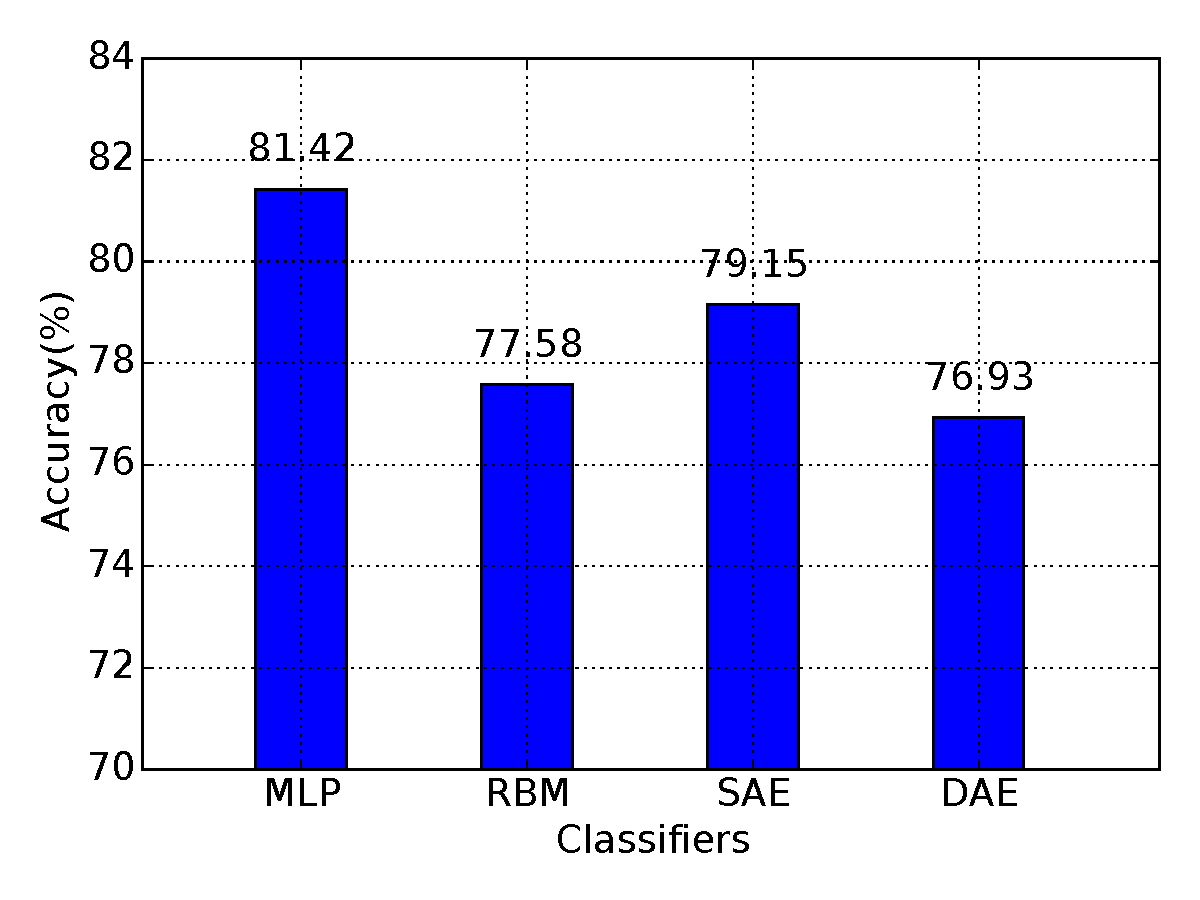
\includegraphics[width=0.48\textwidth]{figures/comp_accuracy.pdf}
    \caption{Classification Accuracy of Proposed Approaches on NSL-KDD Dataset}
    \label{Fig:CompAccuracy}
\end{figure}

Table~\ref{Tab:ConfusionMatrixMLP} --~\ref{Tab:ConfusionMatrixDAE} summarize the confusion matrices
of each approach and their weighted average metrics (Precision, Recall and F1-Score).
Apart from best accuracy, MLP also achieved the best F1-Score (80.44\%)
among all of the considered approaches.
However, we can see that for U2R attacks, MLP still has very poor results of
both precision (13.95\%) and recall (10.35\%).
The second highest F1-Score is achieved by sparse autoencoder combined with softmax regression (78.05\%).
This value is actually a little bit higher than the result (75.76\%) reported in~\cite{STL-NIDS}.
We believe this is partly due to the reason that we did not introduce regularization
for both sparse autoencoder and softmax regression classifier,
and partly due to the dropout technique we used in training the softmax regression classifier.
RBM and DAE again achieve very similar classification performance,
with F1-Score of 75.63\% and 75.65\% respectively.
Considering both the high accuracy and best F1-Score, we conclude that in the competition of
5-class classification, MLP is the winner.

Confusion matrices here tell us something interesting about the classification performance
for each type of traffics.
MLP correctly recognized the most number of normal traffics (9329 out of 9711).
For the attacking traffics, the winner classifier MLP correctly predicted the most
number of DoS attacks (6146 out of 7636), U2R attacks (41 out of 396)
and R2L attacks (926 out of 2376).
RBM is the best classifier in predicting Probe attacks (2015 out of 2425).


\begin{table}[t]
    \caption{Confusion Matrix of MLP on Test Dataset}
    \centering
    \begin{tabular}{cc|rrrrr}
        \hline
        &  & \multicolumn{5}{c}{Prediction} \\
                        &        & Normal & Probe & DoS & U2R & R2L\\
        \hline
        \hline
        \multirow{5}{*}{Actual} & Normal & {\color{red}9329} &  230 &   70 &  25 &  57 \\
                                &  Probe &  164 & 1914 &  271 &  10 &  66 \\
                                &  DoS   & 1358 &   82 & {\color{red}6146} &  47 &   3 \\
                                &  U2R   &  345 &    4 &    0 &  {\color{red}41} &   6 \\
                                &  R2L   & 1247 &   30 &    2 & 171 & {\color{red}926} \\
        \hline
        \multicolumn{2}{c|}{Precision(\%)}   & 74.97 & 84.69 & 94.71 & 13.95 & 87.52\\
        \multicolumn{2}{c|}{Wtd. Avg.(\%)}   & \multicolumn{5}{r}{82.96}\\
        \hline
        \multicolumn{2}{c|}{Recall(\%)}      & 96.07 & 78.93 & 80.49 & 10.35 & 38.97\\
        \multicolumn{2}{c|}{Wtd. Avg.(\%)}   & \multicolumn{5}{r}{81.42}\\
        \hline
        \multicolumn{2}{c|}{F1-Score(\%)}    & 84.22 & 81.71 & 87.02 & 11.88 & 53.93\\
        \multicolumn{2}{c|}{Wtd. Avg.(\%)}   & \multicolumn{5}{r}{\textbf{\color{red}80.44}}\\
        \hline
    \end{tabular}
    \label{Tab:ConfusionMatrixMLP}
\end{table}


\begin{table}[t]
    \caption{Confusion Matrix of RBM on Test Dataset}
    \centering
    \begin{tabular}{cc|rrrrr}
        \hline
        &  & \multicolumn{5}{c}{Prediction} \\
                        &        & Normal & Probe & DoS & U2R & R2L\\
        \hline
        \hline
        \multirow{5}{*}{Actual} & Normal & 8903 &  318 &  428 &  11 &   51 \\
                                & Probe  &  232 & {\color{red}2015} &  159 &   2 &   17 \\
                                & DoS    & 1879 &  143 & 5613 &   0 &    1 \\
                                & U2R    &  356 &    3 &    1 &  27 &    9 \\
                                & R2L    & 1550 &    8 &    1 &   8 &  809 \\
        \hline
        \multicolumn{2}{c|}{Precision(\%)}   & 68.91& 81.02& 90.50& 56.25& 91.21\\
        \multicolumn{2}{c|}{Wtd. Avg.(\%)}   & \multicolumn{5}{r}{79.65}\\
        \hline
        \multicolumn{2}{c|}{Recall(\%)}      & 91.68& 83.09& 73.51&  6.82& 34.05\\
        \multicolumn{2}{c|}{Wtd. Avg.(\%)}   & \multicolumn{5}{r}{77.04}\\
        \hline
        \multicolumn{2}{c|}{F1-Score(\%)}    & 78.68& 82.04& 81.12& 12.16& 49.59\\
        \multicolumn{2}{c|}{Wtd. Avg.(\%)}   & \multicolumn{5}{r}{75.63}\\
        \hline
    \end{tabular}
    \label{Tab:ConfusionMatrixRBM}
\end{table}

\begin{table}[t]
    \caption{Confusion Matrix of SAE on Test Dataset}
    \centering
    \begin{tabular}{cc|rrrrr}
        \hline
        &  & \multicolumn{5}{c}{Prediction} \\
                        &        & Normal & Probe & DoS & U2R  & R2L\\
        \hline
        \hline
        \multirow{5}{*}{Actual}  & Normal & 8864 &  696 &   92 &   11 &   48 \\
                                 & Probe  &  179 & 2001 &  164 &    2 &   79 \\
                                 & DoS    & 1542 &   39 & 6054 &    0 &    1 \\
                                 & U2R    &  357 &    1 &    1 &   30 &    7 \\
                                 & R2L    & 1444 &    6 &    5 &   26 &  895 \\
        \hline
        \multicolumn{2}{c|}{Precision(\%)}    & 71.56& 72.95& 95.85& 43.48& 86.89\\
        \multicolumn{2}{c|}{Wtd. Avg.(\%)}    & \multicolumn{5}{r}{81.06}\\
        \hline
        \multicolumn{2}{c|}{Recall(\%)}       & 91.28& 82.52& 79.28&  7.58& 37.67\\
        \multicolumn{2}{c|}{Wtd. Avg.(\%)}    & \multicolumn{5}{r}{79.15}\\
        \hline
        \multicolumn{2}{c|}{F1-Score(\%)}     & 80.23& 77.44& 86.78& 12.90& 52.55\\
        \multicolumn{2}{c|}{Wtd. Avg.(\%)}    & \multicolumn{5}{r}{78.05}\\
        \hline
    \end{tabular}
    \label{Tab:ConfusionMatrixSAE}
\end{table}


\begin{table}[t]
    \caption{Confusion Matrix of DAE on Test Dataset}
    \centering
    \begin{tabular}{cc|rrrrr}
        \hline
        &  & \multicolumn{5}{c}{Prediction} \\
                        &        & Normal & Probe & DoS & U2R & R2L\\
        \hline
        \hline
        \multirow{5}{*}{Actual} & Normal & 9249 &  319 &   85 &  10 &  48 \\
                                & Probe  & 576  & 1504 &  226 &   2 & 117 \\
                                & DoS    & 1842 &  128 & 5665 &   0 &   1 \\
                                & U2R    & 353  &    1 &    0 &  38 &   4 \\
                                & R2L    & 1469 &    3 &    1 &  17 & 886 \\
        \hline
        \multicolumn{2}{c|}{Precision(\%)} & 68.57& 76.93& 94.78& 56.72& 83.90\\
        \multicolumn{2}{c|}{Wtd. Avg.(\%)} & \multicolumn{5}{r}{79.75}\\
        \hline
        \multicolumn{2}{c|}{Recall(\%)}    & 95.24& 62.02& 74.19&  9.60& 37.29\\
        \multicolumn{2}{c|}{Wtd. Avg.(\%)} & \multicolumn{5}{r}{76.93}\\
        \hline
        \multicolumn{2}{c|}{F1-Score(\%)}  & 79.73& 68.68& 83.23& 16.41& 51.63\\
        \multicolumn{2}{c|}{Wtd. Avg.(\%)} & \multicolumn{5}{r}{75.65}\\
        \hline
    \end{tabular}
    \label{Tab:ConfusionMatrixDAE}
\end{table}
\subsection{Performance of Deep Learning Approaches on UNSW Dataset} 
We plot the prediction accuracies of different approaches in Figure~\ref{Fig:CompAccuracyUNSW}.
Support vector machine (SVM) is adopted as traditional machine learning approach that multiple neural networks compare to.
We trained both linear SVM and non-linear radial basis fuction SVMs and here report the non-linear one's
accuracy on test dataset because it is superior to linear one (81.50\% v.s. 82.25\%).
We also trained a plain neural network of a three layer perceptron with layer size of [480, 512, 640],
denoted as Baseline Neural Network (BL-NN) in the following text.
We use embedding to convert the sparse features in UNSW dataset, listed in Table~\ref{Tab:SparseFeatures}.
Its accuracy, more than 5\% increase to SVM, also serves as baseline for the following two novel models proposed
by deep learning community and described in Section~\ref{Sec:Architectures}.
\begin{table}[]
\centering
\caption{Features Embeddings for the Three-Layer Perceptron}
\label{Tab:SparseFeatures}
\begin{tabular}{c|r|r}
Featue Name & \multicolumn{1}{c|}{Vocabulary Size} & \multicolumn{1}{c}{Embedding Size} \\
\hline
\hline
state       & 11                                  & 4                                  \\
service     & 13                                  & 4                                  \\
protocol    & 133                                 & 8                                 
\end{tabular}
\end{table}

The first model is auxiliary-classifier generative adversarial net (AC-GAN).
Its training contains two phases. In the first stage, we trained an AC-GAN to generate fake
normal and attacking traffics that equals the amount of normal and attacks in training set respectively.
Then we train a single 400-neuron hidden-layer perceptron with both the synthesized and authentic data.
Unfortunately, comparing to the baseline three-layer neural network, AC-GAN does not provide any significant
improvement in terms of accuracy.

The second model we attempted is wide and deep learning model.
As stated in Section~\ref{SubSec:WD}, the wide and deep model (W\&D) requires us engineering the features in UNSW dataset into
basis, crossed, continuous, indicator and embedded features.
The basis features are all the symbolic and integer features.
These basis features are also fed to the deep model after conduct the embedding.
The continuous features are all the float number features.
We make all the combinations of symbolic features to be crossed features.
For comparison reason, we set the structure of the deep neural network in W\&D to be the same sizes as
that of the baseline neural network, namely three hidden layers with sizes of [480, 512, 640].
As the result shows, augmenting the deep neural network with wide linear regressor with non-linear transformed features
provides a 3\% increase in accuracy to the baseline three-layer neural network.

\begin{figure}[h]
    \centering
    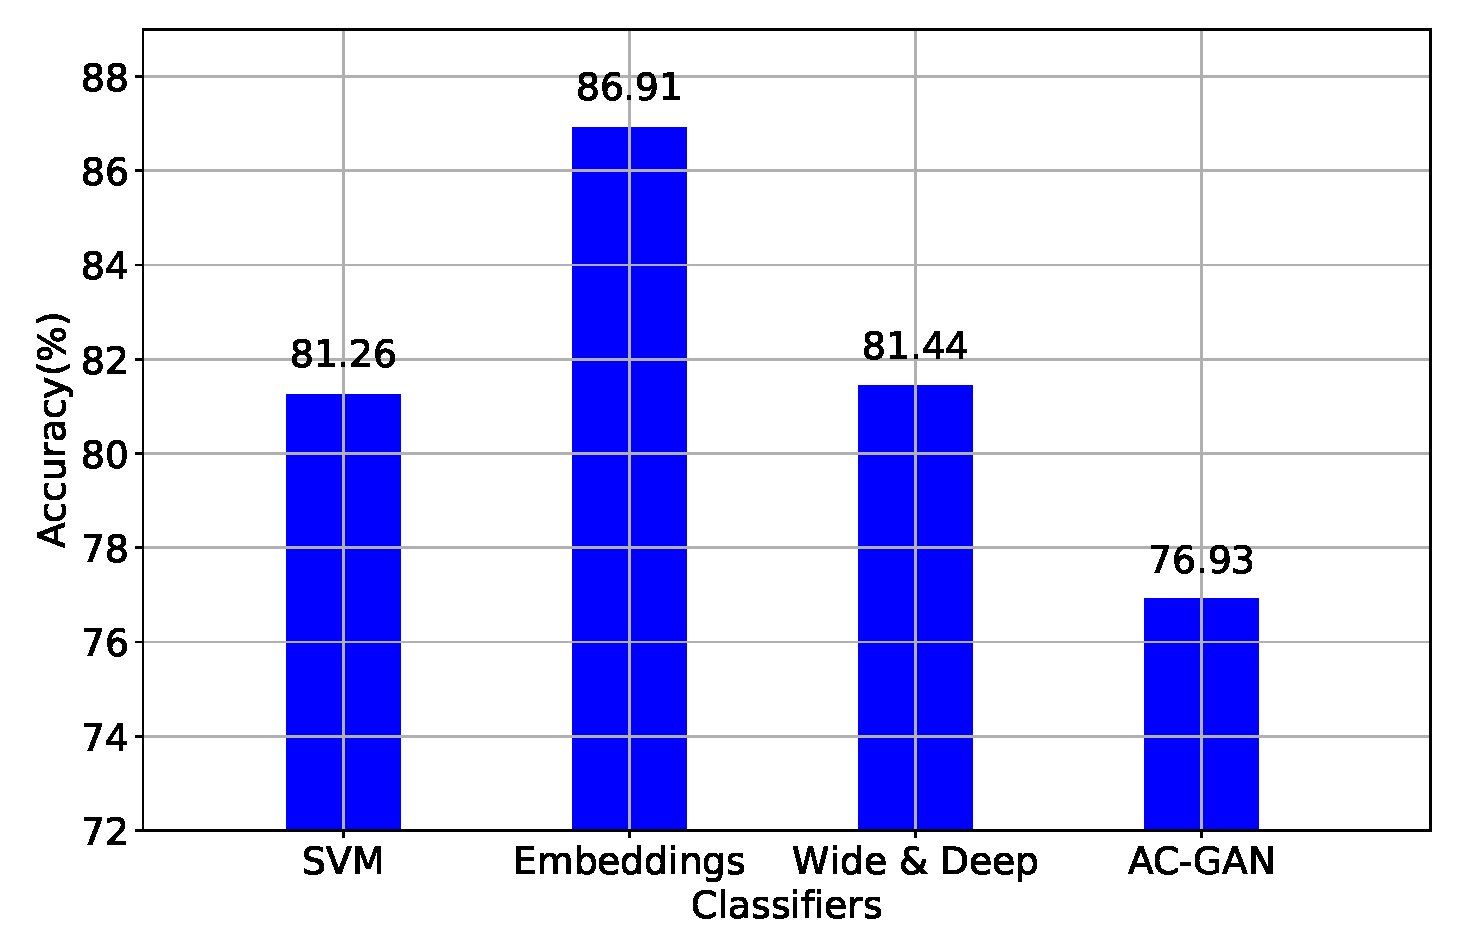
\includegraphics[width=0.48\textwidth]{figures/comp_accuracy_unsw.pdf}
    \caption{Classification Accuracy of Proposed Approaches on UNSW-NB15 Dataset}
    \label{Fig:CompAccuracyUNSW}
\end{figure}


\section{Conclusion}
In this project we conducted a comparative study on the deep learning approaches
for the network intrusion detection problem.
We take the off-line network intrusion detection dataset NSL-KDD for evaluation.
In this paper, multilayer perceptron, restricted Boltzmann machine, sparse autoencoder
and denoising autoencoder are briefly described.
The main contribution lies on sharing the hacks and tricks used in training these neural networks
and the results of comparable evaluation of them.
From our experiment results, we conclude that for the NSL-KDD test dataset,
multilayer perceptron has relatively best performance since both its accuracy and F1-Score
are outstanding among compared neural networks.

\section*{Acknowledgment}
The authors would like to thank...



% An example of a floating figure using the graphicx package.
% Note that \label must occur AFTER (or within) \caption.
% For figures, \caption should occur after the \includegraphics.
% Note that IEEEtran v1.7 and later has special internal code that
% is designed to preserve the operation of \label within \caption
% even when the captionsoff option is in effect. However, because
% of issues like this, it may be the safest practice to put all your
% \label just after \caption rather than within \caption{}.
%
% Reminder: the "draftcls" or "draftclsnofoot", not "draft", class
% option should be used if it is desired that the figures are to be
% displayed while in draft mode.
%
%\begin{figure}[!t]
%\centering
%\includegraphics[width=2.5in]{myfigure}
% where an .eps filename suffix will be assumed under latex, 
% and a .pdf suffix will be assumed for pdflatex; or what has been declared
% via \DeclareGraphicsExtensions.
%\caption{Simulation results for the network.}
%\label{fig_sim}
%\end{figure}

% Note that the IEEE typically puts floats only at the top, even when this
% results in a large percentage of a column being occupied by floats.


% An example of a double column floating figure using two subfigures.
% (The subfig.sty package must be loaded for this to work.)
% The subfigure \label commands are set within each subfloat command,
% and the \label for the overall figure must come after \caption.
% \hfil is used as a separator to get equal spacing.
% Watch out that the combined width of all the subfigures on a 
% line do not exceed the text width or a line break will occur.
%
%\begin{figure*}[!t]
%\centering
%\subfloat[Case I]{\includegraphics[width=2.5in]{box}%
%\label{fig_first_case}}
%\hfil
%\subfloat[Case II]{\includegraphics[width=2.5in]{box}%
%\label{fig_second_case}}
%\caption{Simulation results for the network.}
%\label{fig_sim}
%\end{figure*}
%
% Note that often IEEE papers with subfigures do not employ subfigure
% captions (using the optional argument to \subfloat[]), but instead will
% reference/describe all of them (a), (b), etc., within the main caption.
% Be aware that for subfig.sty to generate the (a), (b), etc., subfigure
% labels, the optional argument to \subfloat must be present. If a
% subcaption is not desired, just leave its contents blank,
% e.g., \subfloat[].


% An example of a floating table. Note that, for IEEE style tables, the
% \caption command should come BEFORE the table and, given that table
% captions serve much like titles, are usually capitalized except for words
% such as a, an, and, as, at, but, by, for, in, nor, of, on, or, the, to
% and up, which are usually not capitalized unless they are the first or
% last word of the caption. Table text will default to \footnotesize as
% the IEEE normally uses this smaller font for tables.
% The \label must come after \caption as always.
%
%\begin{table}[!t]
%% increase table row spacing, adjust to taste
%\renewcommand{\arraystretch}{1.3}
% if using array.sty, it might be a good idea to tweak the value of
% \extrarowheight as needed to properly center the text within the cells
%\caption{An Example of a Table}
%\label{table_example}
%\centering
%% Some packages, such as MDW tools, offer better commands for making tables
%% than the plain LaTeX2e tabular which is used here.
%\begin{tabular}{|c||c|}
%\hline
%One & Two\\
%\hline
%Three & Four\\
%\hline
%\end{tabular}
%\end{table}


% Note that the IEEE does not put floats in the very first column
% - or typically anywhere on the first page for that matter. Also,
% in-text middle ("here") positioning is typically not used, but it
% is allowed and encouraged for Computer Society conferences (but
% not Computer Society journals). Most IEEE journals/conferences use
% top floats exclusively. 
% Note that, LaTeX2e, unlike IEEE journals/conferences, places
% footnotes above bottom floats. This can be corrected via the
% \fnbelowfloat command of the stfloats package.



% conference papers do not normally have an appendix



%% use section* for acknowledgment
%\ifCLASSOPTIONcompsoc
  %% The Computer Society usually uses the plural form
  %\section*{Acknowledgments}
%\else
  %% regular IEEE prefers the singular form
  %\section*{Acknowledgment}
%\fi
%The authors would like to thank...





% trigger a \newpage just before the given reference
% number - used to balance the columns on the last page
% adjust value as needed - may need to be readjusted if
% the document is modified later
%\IEEEtriggeratref{8}
% The "triggered" command can be changed if desired:
%\IEEEtriggercmd{\enlargethispage{-5in}}

% references section

% can use a bibliography generated by BibTeX as a .bbl file
% BibTeX documentation can be easily obtained at:
% http://mirror.ctan.org/biblio/bibtex/contrib/doc/
% The IEEEtran BibTeX style support page is at:
% http://www.michaelshell.org/tex/ieeetran/bibtex/
\bibliographystyle{IEEEtran}
% argument is your BibTeX string definitions and bibliography database(s)
\bibliography{IEEEabrv,ref}
%
% <OR> manually copy in the resultant .bbl file
% set second argument of \begin to the number of references
% (used to reserve space for the reference number labels box)
%\begin{thebibliography}{1}
%\bibitem{IEEEhowto:kopka}
%H.~Kopka and P.~W. Daly, \emph{A Guide to \LaTeX}, 3rd~ed.\hskip 1em plus
%  0.5em minus 0.4em\relax Harlow, England: Addison-Wesley, 1999.
%\end{thebibliography}




% that's all folks
\end{document}


